\part{Lösungen}
\chapter{Grundlagen}
\section{Mengen}
\subsection{Lösung zu Aufgabe~\ref{exc:Aufgabe_1_1}}
Für die Aufgabenstellung siehe Aufgabe~\vref{exc:Aufgabe_1_1}. Für die Lösung der Aufgabe siehe Abbildung~\vref{fig:Loesung_zu_Aufgabe_Aufgabe_1_1}.
\label{loe:Aufgabe_1_1}
\begin{figure}[htb]
\centering
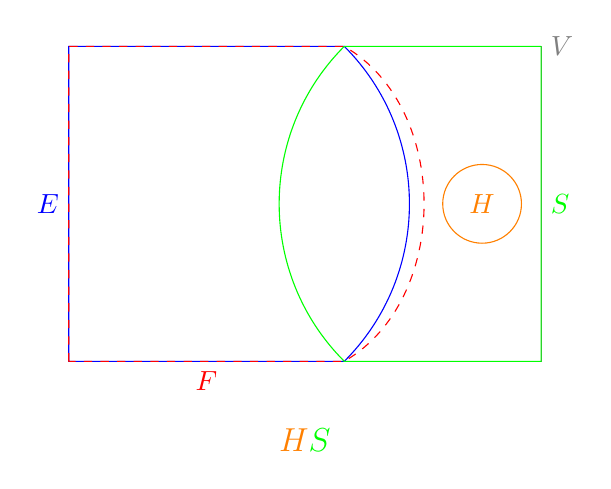
\begin{tikzpicture}
\draw[color=gray] (0,0) rectangle (6,4) node[right] {$V$};
\draw[color=blue] (0,0) -- (0,4) node[left,midway] {$E$} -- (3.5,4) to[out=-45, in=45] (3.5,0) -- (0,0);
\draw[color=red,dashed] (0,0) -- (0,4) -- (3.5,4) to[out=-30, in=30] (3.5,0) -- (0,0) node[below,midway] {$F$};
\draw[color=green] (6,4) -- (3.5,4) to[out=180+45, in=180-45] (3.5,0) -- (6,0) -- (6,4) node[right,midway] {$S$};
\draw[color=orange] (5.25,2) circle(0.5) node {$H$};
\node at (3,-1) {\large $\textcolor{orange}{H} \klgl \textcolor{green}{S}$};
\end{tikzpicture}

\caption{Lösung zu Aufgabe~\ref{exc:Aufgabe_1_1}}
\label{fig:Loesung_zu_Aufgabe_Aufgabe_1_1}
\end{figure}

\section{Logik}
\subsection{Lösung zu Aufgabe~\ref{exc:Aufgabe_1_2}}
Für die Aufgabenstellung siehe Aufgabe~\vref{exc:Aufgabe_1_2}.
\label{loe:Aufgabe_1_2}
\begin{enumerate}
\item $\rk{A \oder B} \und \neg A$ siehe Tabelle~\vref{loe:Aufgabe_1_2_a}.
	\begin{table}[htb]
	\center
	\begin{tabular}{c|c||c|c|c}
	$A$ & $B$ & $A \oder B$ & $\neg A$ & $\rk{A \oder B} \und \neg A$\\\hline
	$w$ & $w$ & $w$ & $f$ & $f$\\
	$w$ & $f$ & $w$ & $f$ & $f$\\
	$f$ & $w$ & $w$ & $w$ & $w$\\
	$f$ & $f$ & $f$ & $w$ & $f$\\
	\end{tabular}
	\caption{Lösung zu Aufgabe~\ref{exc:Aufgabe_1_2} Nummer~\ref{exc:Aufgabe_1_2_a}.}
	\label{loe:Aufgabe_1_2_a}
	\end{table}
\item $\rk{A \und B} \oder \neg A$ siehe Tabelle~\vref{loe:Aufgabe_1_2_b}.
	\begin{table}[htb]
	\center
	\begin{tabular}{c|c||c|c|c}
	$A$ & $B$ & $A \und B$ & $\neg A$ & $\rk{A \und B} \oder \neg A$\\\hline
	$w$ & $w$ & $w$ & $f$ & $w$\\
	$w$ & $f$ & $f$ & $f$ & $f$\\
	$f$ & $w$ & $f$ & $w$ & $w$\\
	$f$ & $f$ & $f$ & $w$ & $w$\\
	\end{tabular}
	\caption{Lösung zu Aufgabe~\ref{exc:Aufgabe_1_2} Nummer~\ref{exc:Aufgabe_1_2_b}.}
	\label{loe:Aufgabe_1_2_b}
	\end{table}
\item $\rk{\neg A \oder \neg B} \und A$ siehe Tabelle~\vref{loe:Aufgabe_1_2_c}.
	\begin{table}[htb]
	\center
	\begin{tabular}{c|c||c|c}
	$A$ & $B$ & $\neg A \oder \neg B$ & $\rk{\neg A \oder \neg B} \oder A$\\\hline
	$w$ & $w$ & $f$ & $f$\\
	$w$ & $f$ & $w$ & $w$\\
	$f$ & $w$ & $w$ & $f$\\
	$f$ & $f$ & $w$ & $f$\\
	\end{tabular}
	\caption{Lösung zu Aufgabe~\ref{exc:Aufgabe_1_2} Nummer~\ref{exc:Aufgabe_1_2_c}.}
	\label{loe:Aufgabe_1_2_c}
	\end{table}
\end{enumerate}

\subsection{Lösung zu Aufgabe~\ref{exc:Aufgabe_1_3}}
Für die Aufgabenstellung siehe Aufgabe~\vref{exc:Aufgabe_1_3}.
\label{loe:Aufgabe_1_3}
\begin{enumerate}
\item \begin{align*}
	&A: \frac{18}{12} (f), B: \frac{18}{3} (w)\\
	&A \Ra B (w)
	\end{align*}

\item \begin{align*}
	&A: \frac{8}{3} (f), B: 14 \in \mathbb{P} (f)\\
	&A \Lra B (w)
	\end{align*}
\end{enumerate}

\section{Relationen und Abbildungen}
\subsection{Lösung zu Aufgabe~\ref{exc:Aufgabe_1_4}}
Für die Aufgabenstellung siehe Aufgabe~\vref{exc:Aufgabe_1_4}.
\label{loe:Aufgabe_1_4}

\chapter{Übungsblätter}
\section{Übungsblatt 1}
\subsection{Aufgabe 1.2}
$A, B \subseteq G$
\begin{enumerate}[label=\alph*)]
\item \ac{z.z.} $A \subseteq B \Lra A \cap \bar{B} = \emptyset$\\
	\begin{align*}
	&A \subseteq B\\
	\Lra & \rk{x \in A \Ra x \in B}\\
	\Lra & \rk{x \notin B \Ra x \notin A}\\
	\Lra & \rk{x \in \bar{B} \Ra x \notin A}\\
	\Lra & \notexists x \in \bar{B} \cap A\\
	\Lra & A \cap \bar{B} = \emptyset
	\end{align*}

\item $A \subseteq B \Lra \bar{A} \cup B = G$
	\begin{align*}
	&A \subseteq B\\
	\Lra & A \cap \bar{B} = \emptyset\\
	\Lra & \overline{\rk{A \cap \bar{B}}} = \bar{\emptyset}\\
	\Lra & \bar{A} \cup B = G
	\end{align*}
\end{enumerate}

\subsection{Aufgabe 1.3}
\begin{enumerate}[label=\alph*)]
\item $T$ = Menge aller Tiere, $P$ = Menge aller Pflanzen\\
	$\neg\rk{\tx{Alle Tiere haben Beine oder Flossen und alle Pfalnzen haben Wurzeln}}$\\
	$\Lra \neg\rk{\rk{\forall x \in T: x \tx{ hat Beine } \oder x \tx{ hat Flossen}} \und \rk{\forall y \in P: y \tx{ hat Wurzeln}}}$\\
	$\Lra \neg\rk{\forall x \in T: x \tx{ hat Beine } \oder x \tx{ hat Flossen} \oder \neg\rk{\forall y \in P: y \tx{ hat Wurzeln}}}$\\
	$\Lra \rk{\exists x \in T: x \tx{ hat keine Beine } \und x \tx{ hat keine Flossen}} \oder \rk{\exists y \in P: y \tx{ hat keine Wurzeln}}$\\
	$\Lra$ Es gibt mindestens ein Tier, das weder Beine noch Flossen hat oder es gibt \ac{mind.} eine Pflanze ohne Wurzeln.

\item $A_1$ = Menge aller Arbeitnehmer, die mehr als 400- verdienen, $A_2$ = Menge aller Arbeitnehmer mit mehr als einem Arbeitsverhältnis\\
	$\neg$(Alle Arbeitnehmer, die mehr als 400-/Monat verdienen oder mehr als ein Arbeitsverhältnis haben, zahlen Lohnsteuer)\\
	$\Lra \neg\rk{\forall x \in A_1 \cup A_2: x \tx{ zahlt Lohnsteuer}}$\\
	$\Lra \exists x \in A_1 \cup A_2: x \tx{ zahlt keine Lohnsteuer}$\\
	$\Lra$ Es gibt \ac{mind.} ein Arbeitnehmer, der mehr als 400-/Monat verdient oder mehr als ein Arbeitsverhältnis hat, der keine Lohnsteuer zahlt

\item $K$ = Menge aller Käfer, $M$ = Menge aller Fledermäuse, $L$ = Menge aller Landtiere, $F$ = Menge aller Fische\\
	$\neg$ (Es \ac{ex.} \ac{mind.} ein Käfer oder eine Fledermaus, die schneller ist als alle Fische und Landtiere)\\
	$\Lra \neg\rk{\exists x \in K \cup M: x \tx{ ist schneller als alle } y \in F \cup L}$\\
	$\Lra \forall x \in K \cup M: \neg\rk{x \tx{ ist schneller als alle } y \in F \cup L}$\\
	$\Lra \forall x \in K \cup M: \exists y \in F \cup L \tx{ mit } y \tx{ ist \ac{mind.} so schnell wie } x$\\
	$\Lra$ Es gibt \ac{mind.} ein Fisch oder Landtier, das \ac{mind.} ebenso schnell ist wie alle Käfer und Fledermäuse.
\end{enumerate}

\subsection{Aufgabe 1.4}
\begin{enumerate}[label=\alph*)]
\item $A_1 = \Z$, $\rk{x, y} \in R_1 \Lra x + y \tx{ ist ungerade}$
	\begin{description}
	\item[nicht reflexiv] $x + x = 2x$ gerade $\Ra \rk{x, x} \notin R_1$
	\item[symmetrisch] $\rk{x, y} \in R_1$
		\begin{align*}
		\Lra& x + y \tx{ ungerade}\\
		\Lra& y + x\\
		\Lra& \rk{y, x} \in R_1
		\end{align*}

	\item[nicht antisymmetrisch] $\rk{1, 2} \in R_1 \und \rk{2, 1} \in R_1 \tx{ aber } 1 \neq 2$
	\item[nicht transitiv] \ac{z.B.} $\rk{1, 2} \in R_1 \und \rk{2, 1} \in R_1 \tx{ aber } \rk{1, 1} \notin R_1$
	\item[nicht vollständig] da nicht reflexiv, beispielsweise $\rk{1, 1} \notin R_1$
	\end{description}

\item $A_2 = \Z$, $\rk{x, y} \in R_2 \Lra x + y \tx{ gerade}$
	\begin{description}
	\item[reflexiv] $x + x = 2x$ gerade $\Ra \rk{x, x} \in R_2$
	\item[symmetrisch] $\rk{x, y} \in R_2 \Lra x + y$ gerade $\Lra y + x$ gerade $\Lra \rk{y, x} \in R_2$
	\item[nicht antisymmetrisch] $\rk{1, 3} \in R_2 \und \rk{3, 1} \in R_2$ aber $1 \neq 3$
	\item[transitiv] \ac{z.z.} $\rk{x, y} \in R_2 \und \rk{y, z} \in R_2 \Ra \rk{x, z} \in R_2$\\
		Fall 1/\textcolor{blue}{2}
		\begin{align*}
		&x \tx{ungerade/\textcolor{blue}{gerade}} \und \rk{x, y} \in R_2\\
		\Lra & x \tx{ungerade/\textcolor{blue}{gerade}} \und y \tx{ungerade/\textcolor{blue}{gerade}}\\
		&y \tx{ungerade/\textcolor{blue}{gerade}} \und \rk{y, z} \in R_2\\
		\Lra& y \tx{ungerade/\textcolor{blue}{gerade}} \und z \tx{ungerade/\textcolor{blue}{gerade}}\\
		\Ra& x + z \tx{ gerade } \Lra \rk{x, z} \in R_2
		\end{align*}

	\item[nicht vollständig] $\rk{1, 2} \notin R_2 \und \rk{2, 1} \notin R_2$
	\end{description}

\item $A_3 = \Z$, $\rk{x, y} \in R_3 \Lra xy \tx{ ungerade}$
	\begin{description}
	\item[nicht reflexiv] $2 \mal 2 = 4$ gerade $\Ra \rk{2,2} \notin R_3$
	\item[symmetrisch] $\rk{x, y} \in R_3 \Lra x \mal y$ ungerade $\Lra y \mal x$ ungerade $\Lra \rk{y, x} \in R_3$
	\item[nicht antisymmetrisch] $\rk{1, 3} \in R_3 \und \rk{3, 1} \in R_3$ aber $1 \neq 3$
	\item[transitiv] $\rk{x, y} \in R_3 \und \rk{y, z} \in R_3$
		\begin{align*}
		&\Lra x \mal y \tx{ ungerade } \und y \mal z \tx{ ungerade}\\
		&\Lra x, y, z \tx{ ungerade}\\
		&\Ra x \mal z \tx{ ungerade } \Lra \rk{x, z} \in R_3
		\end{align*}

	\item[nicht vollständig] da nicht reflexiv
	\end{description}

\item $A_4 = \Z$ $\rk{x, y} \in R_4 \Lra x + x \mal y$ gerade
	\begin{description}
	\item[reflexiv] $x + x \mal x = \ub{x \rk{1 + x}}{\tx{gerade}}$ da immer entweder $x$ gerade oder $x + 1$ gerade $\Lra \rk{x, x} \in R_4$
	\item[nicht symmetrisch] $x \rk{1 + y}$\\
		$\rk{2, 1} \in R_4 \rk{\Lra 2 \mal \rk{1 + 1} = 4}$\\
		$\rk{1, 2} \notin R_4 \rk{\Lra 1 \rk{1 + 2} = 3}$

	\item[nicht antisymmetrisch] $\rk{2, 4} \in R_4 \und \rk{4, 2} \in R_4$ aber $2 \neq 4$
	\item[transitiv]
		\begin{description}
		\item[Fall 1] $x$ gerade, $\rk{x, y} \in R_4 \oder \rk{y, z} \in R_4$\\
			$x \rk{1 + y}$ gerade\\
			$x \rk{1 + z}$ gerade\\
			$\Ra \rk{x, z} \in R_4$

		\item[Fall 2] $x$ ungerade, $\rk{x, y} \in R_4 \und \rk{y, z} \in R_4$
			\begin{itemize}
			\item $x \rk{1 + y}$ gerade, $x$ ungerade $\Ra y$ ungerade
			\item $y \rk{1 + z}$ gerade, $y$ ungerade $\Ra z$ ungerade
			\end{itemize}
			$\Ra x \ub{\rk{1 + z}}{\tx{gerade}}$ gerade $\Lra \rk{x, z} \in R_4$
		\end{description}

	\item[vollständig] \ac{z.z.} $\rk{x, y} \in R_4 \oder \rk{y, x} \in R_4$
		\begin{description}
		\item[Fall 1] $x$ gerade
		\end{description}
	\end{description}
\end{enumerate}